\subsection*{Edificio Principal del Aeropuerto Jorge Chavez}
%\phantomsubsection
\addcontentsline{toc}{subsection}{Edificio Principal del Aeropuerto Jorge Chavez}

La \autoref{Anexo_1} muestra las histéresis de uno de los dos los DFV instalados en el eje 5-5 del primer nivel del edificio pincipal del aeropuerto Jorge Chavez. Asimismo, la \autoref{Anexo_2} presenta la histéresis de uno de los tres DH-SLB colocado en el eje 5-5 del primer nivel de la misma edificación.


	\begin{figure}[!h]
	\centering
	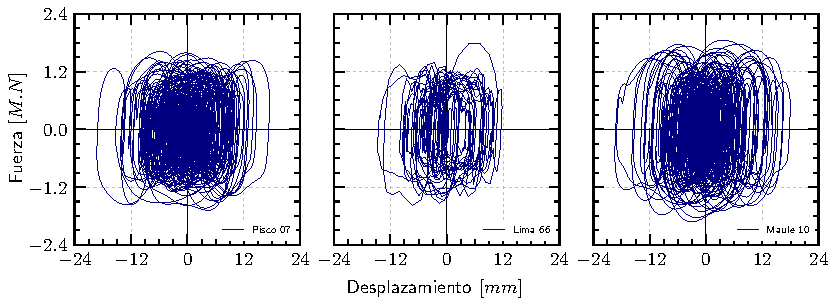
\includegraphics[scale=1]{E_IMAGENES/Anexos/Anexo_1.pdf}
	\vspace{-8 mm}
	\caption[]{\centering\footnotesize Histéresis del DFV del edificio del aeropuerto Jorge Chavez.}
	\label{Anexo_1}
	\end{figure}	


	\begin{figure}[!h]
	\centering
	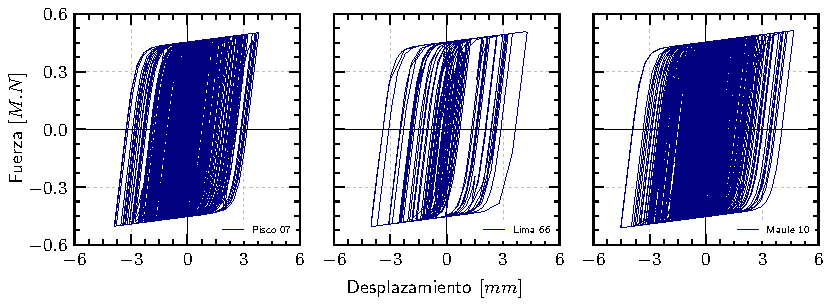
\includegraphics[scale=1]{E_IMAGENES/Anexos/Anexo_2.pdf}
	\vspace{-8 mm}
	\caption[]{\centering\footnotesize Histéresis del DH-SLB del edificio del aeropuerto Jorge Chavez.}
	\label{Anexo_2}
	\end{figure}	
